\documentclass[11pt]{article}
\usepackage[margin=1in]{geometry}
\usepackage{booktabs}
\usepackage{graphicx}
\usepackage{amsmath,amssymb}
\usepackage{hyperref}
\usepackage{xcolor}
\usepackage{caption}
\usepackage{array}
\usepackage{multirow}

\hypersetup{colorlinks=true, linkcolor=blue, citecolor=blue, urlcolor=blue}

\title{Endogenous Preference Dynamics in News Consumption:\\[6pt]
\large Evidence from 750K Users over 14 Days}
\author{UBC Gang}
\date{April 2026}

\begin{document}
\maketitle

\begin{abstract}
Do users' preferences shift in response to what they consume---and does it matter whether they actively engage or merely see the content? We study these questions using the Microsoft MIND Large dataset (750K users, 5M impressions, November 9--22, 2019). A three-period design---baseline, treatment, outcome---reveals two main findings. First, consumption reshapes taste: what users click in the middle period predicts the direction of their taste shift into the late period (cosine alignment $+0.36$, permutation $z = 515$). Self-reinforcement is universal, with a $+243\%$ lift across all 14 content categories. Second, engagement is the mechanism, not exposure. Clicking an article in a category pulls taste toward it (Cohen's $d = 1.13$), but being shown articles without clicking pushes taste \emph{away}---below the baseline of never having been shown the category at all (within-user $d = -0.75$, 13/14 categories). The backfire intensifies with the dose of ignored exposure ($\rho = -0.21$). These findings support a taste transition model in which clicked content reinforces preferences and ignored content erodes them.
\end{abstract}

\section{Data and Design}

The MIND Large dataset comprises three splits of user--article interactions on Microsoft News:

\begin{center}
\begin{tabular}{lccc}
\toprule
Split & Dates & Impressions & Users \\
\midrule
Train & Nov 9--14 & 2,232,748 & 711,222 \\
Dev & Nov 15 & 376,471 & 255,657 \\
Test & Nov 16--22 & 2,370,727 & 702,005 \\
\midrule
\textbf{Total} & \textbf{Nov 9--22} & \textbf{4,979,946} & \textbf{$\sim$1M unique} \\
\bottomrule
\end{tabular}
\end{center}

The test set lacks impression-level click labels (competition format) but retains each user's cumulative click history. A user's test-period history minus their train-period history reveals which articles they clicked during November 16--22. This lets us construct a third observation window where we know \emph{what} was consumed but not what was offered.

We partition the 14-day span into three periods: P1 (Nov 9--11, 869K labeled impressions), P2 (Nov 12--15, 1.74M), and P3 (Nov 16--22, inferred from test history growth for 575K users). Each user's taste in a period is a category-distribution vector $\boldsymbol{\theta} \in \mathbb{R}^{15}$, normalized over 15 content categories from 130,379 unique articles. Users with at least 2 clicks in each period form the analysis sample: 146,478 users.

\section{Taste Persistence}

A user's history strongly predicts what they click next. The cosine similarity between historical taste and current clicks is $0.682$, and the platform exploits this: the alignment between history and \emph{shown} articles is even higher ($0.776$). Users diversify slightly relative to offers---only 34\% click a distribution more concentrated than what the algorithm recommends.

The predictive power of history holds in every category. Users with heavy prior consumption in a category click it at $1.8\times$ to $464\times$ the rate of light consumers (all $p < 10^{-234}$). Niche categories like autos ($7.5\times$) and kids ($464\times$) produce the sharpest taste signals; broad categories like news ($2.0\times$) and music ($1.8\times$) the weakest. The pattern is consistent with a model in which taste persistence governs choice: past consumption reveals stable preferences that predict future behavior.

\section{Taste Shift}
\label{sec:shift}

The three-period structure enables a direct test of whether taste actually moves. It does.

\subsection*{Persistence decays with time}

\begin{center}
\begin{tabular}{lcc}
\toprule
Period pair & Time gap & Cosine similarity \\
\midrule
P1 $\leftrightarrow$ P2 & 1--6 days & 0.525 \\
P2 $\leftrightarrow$ P3 & 1--10 days & 0.884 \\
P1 $\leftrightarrow$ P3 & 5--14 days & 0.827 \\
\bottomrule
\end{tabular}
\end{center}

Taste vectors are correlated across periods but well below 1.0, and the P1--P2 similarity (0.525) is notably lower than P2--P3 (0.884). Part of this reflects noisier estimation in the shorter P1 window, but the decay from P2--P3 to P1--P3 confirms genuine drift over the 14-day horizon.

\subsection*{Consumption predicts the direction of taste shift}

We define the taste shift $\Delta\boldsymbol{\theta} = \boldsymbol{\theta}^{\text{P3}} - \boldsymbol{\theta}^{\text{history}}$ and test its alignment with intermediate consumption.

\begin{center}
\begin{tabular}{lccc}
\toprule
Alignment & Mean $\cos$ & $t$ & $p$ \\
\midrule
$\cos(\text{P2 shift}, \text{P1 consumption})$ & $-0.008$ & $-8.1$ & $4 \times 10^{-16}$ \\
$\cos(\text{P3 shift}, \text{P2 consumption})$ & $\mathbf{+0.360}$ & $\mathbf{429}$ & $< 10^{-300}$ \\
$\cos(\text{P3 shift}, \text{P1+P2 consumption})$ & $+0.397$ & $501$ & $< 10^{-300}$ \\
\bottomrule
\end{tabular}
\end{center}

In the 7-day MINDsmall dataset, which lacked a third period, this alignment was $-0.012$ (insignificant). With 14 days and the test set providing P3, it jumps to $+0.360$ with a permutation $z$-score of 515. What users consume in the middle period predicts where their taste drifts next.

\subsection*{Transition matrix}

Table~\ref{tab:transition} shows P3 category distributions conditional on each user's dominant P1 category. The diagonal dominates: news readers stay with news ($0.46$), sports readers with sports ($0.44$). Off-diagonal flow is asymmetric---most categories leak toward news, the largest category, while news and sports leak the least. Niche categories (entertainment: $0.21$, movies: not shown due to small sample) are the leakiest. These patterns are consistent with a model in which broad categories are absorbing and niche categories are transient.

\begin{table}[ht]
\centering
\caption{Transition matrix: P1 dominant category $\to$ P3 click distribution. Diagonal entries (bold) show self-reinforcement. 143,574 three-period users.}
\label{tab:transition}
\small
\setlength{\tabcolsep}{3.5pt}
\begin{tabular}{l|cccccccccc}
\toprule
& news & sports & fin. & life. & health & trav. & food & autos & ent. & video \\
\midrule
news & \textbf{.46} & .12 & .07 & .08 & .03 & .03 & .03 & .02 & .02 & .02 \\
sports & .17 & \textbf{.44} & .06 & .06 & .02 & .03 & .03 & .02 & .02 & .01 \\
finance & .23 & .12 & \textbf{.26} & .10 & .04 & .03 & .04 & .02 & .02 & .02 \\
lifestyle & .20 & .08 & .05 & \textbf{.33} & .04 & .03 & .04 & .01 & .04 & .02 \\
health & .19 & .09 & .06 & .13 & \textbf{.24} & .03 & .04 & .02 & .03 & .02 \\
travel & .16 & .08 & .07 & .10 & .04 & \textbf{.28} & .04 & .03 & .03 & .02 \\
food & .18 & .08 & .06 & .13 & .05 & .04 & \textbf{.26} & .02 & .03 & .01 \\
autos & .19 & .11 & .08 & .08 & .04 & .04 & .04 & \textbf{.26} & .03 & .02 \\
entert. & .18 & .09 & .06 & .13 & .05 & .03 & .04 & .01 & \textbf{.21} & .02 \\
video & .20 & .06 & .05 & .10 & .03 & .03 & .03 & .02 & .02 & \textbf{.35} \\
\bottomrule
\end{tabular}
\end{table}

\section{Self-Reinforcement}

Clicking an article in a category raises the probability of clicking the same category next. The lift is large and universal:

\begin{center}
\begin{tabular}{lcccc}
\toprule
Category & $P(\text{next}|\text{click})$ & $P(\text{next}|\text{no click})$ & Lift & $p$ \\
\midrule
autos & 0.127 & 0.023 & $+448\%$ & $< 10^{-300}$ \\
video & 0.068 & 0.019 & $+254\%$ & $< 10^{-300}$ \\
foodanddrink & 0.118 & 0.036 & $+232\%$ & $< 10^{-300}$ \\
weather & 0.061 & 0.024 & $+154\%$ & $< 10^{-143}$ \\
health & 0.080 & 0.034 & $+132\%$ & $< 10^{-300}$ \\
travel & 0.058 & 0.026 & $+127\%$ & $< 10^{-234}$ \\
entertainment & 0.077 & 0.035 & $+122\%$ & $< 10^{-300}$ \\
movies & 0.031 & 0.014 & $+123\%$ & $< 10^{-71}$ \\
sports & 0.243 & 0.113 & $+114\%$ & $< 10^{-300}$ \\
lifestyle & 0.193 & 0.105 & $+84\%$ & $< 10^{-300}$ \\
tv & 0.068 & 0.044 & $+53\%$ & $< 10^{-129}$ \\
finance & 0.116 & 0.080 & $+45\%$ & $< 10^{-184}$ \\
news & 0.353 & 0.245 & $+44\%$ & $< 10^{-300}$ \\
music & 0.077 & 0.060 & $+29\%$ & $< 10^{-54}$ \\
\midrule
\textbf{Overall} & \textbf{0.184} & \textbf{0.054} & $\boldsymbol{+243\%}$ & $< 10^{-300}$ \\
\bottomrule
\end{tabular}
\end{center}

All 14 categories are significant. The overall lift of $+243\%$ matches the MINDsmall estimate ($+242\%$) almost exactly, across $10\times$ more users. Niche categories produce the largest lifts because their baseline click rate is low; a single click is a strong signal.

\section{Entropy: Local Reinforcement, Global Diversification}

The self-reinforcement result might suggest that users narrow over time. They do not. Category-level entropy increases monotonically across the three periods:

\begin{center}
\begin{tabular}{lccc}
\toprule
Period & Mean entropy & $\Delta$ from P1 & $t$ \\
\midrule
P1 (Nov 9--11) & 1.352 bits & --- & --- \\
P2 (Nov 12--15) & 1.590 bits & $+0.238$ & $116$ \\
P3 (Nov 16--22) & 2.047 bits & $+0.678$ & $474$ \\
\bottomrule
\end{tabular}
\end{center}

By P3, 90.7\% of users have higher entropy than in P1. At the category level, clicking sports makes you more likely to click sports again. At the portfolio level, users explore new categories over time. The taste vector spreads outward rather than collapsing to a single peak---local reinforcement coexists with global diversification. A taste transition model should preserve the dominant direction while allowing diffusion into adjacent categories.

\section{Controlled Regression}

To separate the effect of history from the mechanical influence of what the platform offers, we regress click fractions on both historical taste and the shown assortment:

\begin{center}
\begin{tabular}{lcccc}
\toprule
Variable & Coef & SE & $t$ & $p$ \\
\midrule
Intercept & $-0.007$ & $<0.001$ & $-93$ & $< 10^{-300}$ \\
hist\_frac & $0.390$ & $<0.001$ & $722$ & $< 10^{-300}$ \\
shown\_frac & $0.695$ & $<0.001$ & $838$ & $< 10^{-300}$ \\
\midrule
\multicolumn{5}{l}{$N = 4{,}958{,}784$, \quad $R^2 = 0.411$} \\
\bottomrule
\end{tabular}
\end{center}

Historical taste predicts clicks ($\beta = 0.39$) even after controlling for the assortment. The inner-product utility model is well-supported: a user's taste vector and the category composition of the offer jointly explain 41\% of click variation across 5M observations.

\section{Robustness: Small vs.\ Large Dataset}

\begin{center}
\begin{tabular}{lcc}
\toprule
& MINDsmall & MINDlarge \\
\midrule
Users analyzed & 35,443 & 378,020 \\
$\cos(\text{hist}, \text{clicked})$ & 0.664 & 0.682 \\
$\cos(\text{hist}, \text{shown})$ & 0.769 & 0.776 \\
Self-reinforcement lift & $+242\%$ & $+243\%$ \\
Categories significant & 14/14 & 14/14 \\
$\beta(\text{hist\_frac})$ & 0.406 & 0.390 \\
$R^2$ & 0.382 & 0.411 \\
\textbf{Taste shift alignment} & $\boldsymbol{-0.012}$ (n.s.) & $\boldsymbol{+0.360}$ ($p < 0.001$) \\
Time window & 7 days & 14 days \\
Three-period users & N/A & 143,574 \\
\bottomrule
\end{tabular}
\end{center}

Every result replicates within 3\%, except the one that requires the longer window: taste shift alignment flips from insignificant ($-0.012$) to highly significant ($+0.360$). The 14-day span and three-period design are essential for detecting directional taste change.


\section{Exposure vs.\ Engagement}
\label{sec:exposure}

Taste drifts toward what users consume. But consumption is shaped by what the platform \emph{shows}. The natural follow-up: does mere exposure move taste, or only active engagement?

In P2 we observe both what was shown and what was clicked. Every (user, category) pair falls into one of three groups: \emph{clicked} (shown and clicked), \emph{shown-not-clicked} (shown but ignored), or \emph{neither} (never shown). The outcome is the taste shift $\Delta_c = \theta_c^{\text{P3}} - \theta_c^{\text{P1}}$. After filtering to users with sufficient activity in all three periods, 145,985 users remain.

\subsection*{Aggregate regression}

A stacked OLS with user-clustered standard errors regresses P3 taste on P1 taste, P2 clicks, and P2 shown composition:

\begin{center}
\begin{tabular}{lcccc}
\toprule
Variable & Coef & SE (clust) & $t$ & $p$ \\
\midrule
Intercept & $0.001$ & $<0.001$ & $28.0$ & $<10^{-300}$ \\
$\theta^{\text{P1}}$ (baseline) & $0.407$ & $0.001$ & $801.7$ & $<10^{-300}$ \\
P2 clicks & $0.521$ & $0.001$ & $945.0$ & $<10^{-300}$ \\
P2 shown & $0.059$ & $0.001$ & $88.5$ & $<10^{-300}$ \\
\midrule
\multicolumn{5}{l}{$N = 1{,}852{,}089$ \quad $N_{\text{clusters}} = 145{,}985$ \quad $R^2 = 0.949$} \\
\bottomrule
\end{tabular}
\end{center}

Baseline taste and clicks dominate ($\beta_1 = 0.41$, $\beta_2 = 0.52$). The shown composition enters positively ($\beta_3 = 0.06$), which might suggest a modest mere-exposure channel. Decomposing that term reveals a different story.

\subsection*{Clicked vs.\ non-clicked exposure}

Replacing the aggregate regressors with \emph{shown-and-clicked} and \emph{shown-and-NOT-clicked} fractions separates engagement from passive exposure:
\[
\theta_{c}^{\text{P3}} \;=\; \beta_0 + \beta_1\,\theta_{c}^{\text{P1}} + \beta_2\,\text{shown{+}clicked}_{c}^{\text{P2}} + \beta_3\,\text{shown{+}NOT clicked}_{c}^{\text{P2}} + \varepsilon.
\]

\begin{center}
\begin{tabular}{lcccc}
\toprule
Variable & Coef & SE (clust) & $t$ & $p$ \\
\midrule
Intercept & $0.001$ & $<0.001$ & $27.4$ & $<10^{-300}$ \\
$\theta^{\text{P1}}$ (baseline) & $0.412$ & $0.001$ & $804.3$ & $<10^{-300}$ \\
Shown + clicked & $\mathbf{0.509}$ & $0.001$ & $998.2$ & $<10^{-300}$ \\
Shown + NOT clicked & $\mathbf{0.067}$ & $0.001$ & $103.9$ & $<10^{-300}$ \\
\midrule
\multicolumn{5}{l}{$N = 1{,}852{,}089$ \quad $N_{\text{clusters}} = 145{,}985$ \quad $R^2 = 0.940$} \\
\bottomrule
\end{tabular}
\end{center}

Clicked exposure is $7.6\times$ as predictive as non-clicked exposure ($0.509$ vs.\ $0.067$). The positive $\beta_3$ might still suggest a weak pure-exposure effect, but the direction-of-shift analysis below overturns that interpretation.

\subsection*{Direction of taste shift}

The cosine similarity between each user's taste shift $\boldsymbol{\Delta} = \boldsymbol{\theta}^{\text{P3}} - \boldsymbol{\theta}^{\text{P1}}$ and four P2 vectors tells us where taste actually moves:

\begin{center}
\begin{tabular}{lcccc}
\toprule
Alignment target & Mean $\cos$ & $t$ & $p$ & Cohen's $d$ \\
\midrule
P2 shown (all) & $+0.026$ & $36.2$ & $<10^{-285}$ & $0.095$ \\
P2 clicks & $+0.375$ & $433.0$ & $<10^{-300}$ & $1.141$ \\
P2 shown + clicked & $+0.372$ & $427.1$ & $<10^{-300}$ & $1.125$ \\
P2 shown + NOT clicked & $\mathbf{-0.015}$ & $-21.2$ & $<10^{-99}$ & $-0.056$ \\
\bottomrule
\end{tabular}
\end{center}

Taste shifts \emph{toward} what users click ($\cos = +0.37$) and \emph{away} from what they see but do not click ($\cos = -0.015$). The paired difference is massive ($t = 457$, $p < 10^{-300}$). The positive aggregate shown-alignment ($+0.026$) is a mixture of these two opposing forces; the clicked component overwhelms the non-clicked component in the aggregate, masking the backfire.

\subsection*{The backfire}

The cleanest test compares mean taste shift across the three exposure groups:

\begin{center}
\begin{tabular}{lcccc}
\toprule
Exposure group & $N$ (pairs) & Mean $\Delta$ & $t$ & $p$ \\
\midrule
Clicked & 578,585 & $+0.056$ & $301.5$ & $<10^{-300}$ \\
Shown, not clicked & 1,257,417 & $-0.024$ & $-366.3$ & $<10^{-300}$ \\
Neither shown nor clicked & 353,773 & $-0.006$ & $-101.2$ & $<10^{-300}$ \\
\bottomrule
\end{tabular}
\end{center}

Clicked categories gain taste share ($+0.056$). Categories never shown drift slightly downward ($-0.006$), a natural consequence of the taste pie being finite. But shown-not-clicked categories decline \emph{four times as much} ($-0.024$)---significantly more than the neither group ($t = -137.7$). Within-user paired comparisons sharpen this: the mean within-user difference between shown-not-clicked and neither is $-0.021$ ($t = -287.0$, Cohen's $d = -0.75$). Exposure without engagement does not merely fail to help---it actively erodes taste.

\subsection*{Dose-response}

The backfire intensifies with the amount of ignored exposure. Among shown-not-clicked (user, category) pairs, Spearman $\rho$ between the shown fraction and the taste shift is $-0.208$ ($p < 10^{-300}$). Binned by quintile:

\begin{center}
\begin{tabular}{ccc}
\toprule
Quintile & Mean shown fraction & Mean $\Delta$ \\
\midrule
1 (lowest) & 0.012 & $-0.008$ \\
2 & 0.028 & $-0.016$ \\
3 & 0.045 & $-0.021$ \\
4 & 0.067 & $-0.026$ \\
5 (highest) & 0.138 & $-0.049$ \\
\bottomrule
\end{tabular}
\end{center}

Users in the top quintile of ignored exposure experience a $6\times$ larger taste decline than those in the bottom quintile. An OLS confirms the gradient: $\Delta = -0.005 - 0.325 \times \text{shown\_frac}$ ($t = -170.5$).

\subsection*{Per-category decomposition}

Table~\ref{tab:percat} reports click and exposure effects for each category. The click effect is positive everywhere ($+0.067$ to $+0.102$). The exposure effect---the taste shift attributable to being shown content without clicking---is negative in 13 of 14 categories. Only sports shows a small positive effect ($+0.009$). News exhibits the largest backfire ($-0.024$), followed by lifestyle ($-0.018$).

\begin{table}[ht]
\centering
\caption{Per-category decomposition. Click effect: clicked $\Delta$ minus neither $\Delta$. Exposure effect: shown-not-clicked $\Delta$ minus neither $\Delta$. Positive values indicate taste reinforcement; negative values indicate backfire.}
\label{tab:percat}
\small
\begin{tabular}{lccccc}
\toprule
Category & Clicked $\Delta$ & Shown-NC $\Delta$ & Neither $\Delta$ & Click eff. & Exposure eff. \\
\midrule
news & $+0.021$ & $-0.105$ & $-0.081$ & $+0.102$ & $-0.024$ \\
sports & $+0.043$ & $-0.045$ & $-0.054$ & $+0.097$ & $+0.009$ \\
lifestyle & $+0.086$ & $-0.028$ & $-0.011$ & $+0.097$ & $-0.018$ \\
finance & $+0.078$ & $-0.025$ & $-0.016$ & $+0.094$ & $-0.009$ \\
weather & $+0.090$ & $-0.004$ & $-0.003$ & $+0.093$ & $-0.001$ \\
music & $+0.059$ & $-0.038$ & $-0.033$ & $+0.092$ & $-0.004$ \\
video & $+0.075$ & $-0.006$ & $-0.003$ & $+0.078$ & $-0.003$ \\
movies & $+0.063$ & $-0.014$ & $-0.010$ & $+0.073$ & $-0.004$ \\
health & $+0.062$ & $-0.019$ & $-0.009$ & $+0.071$ & $-0.010$ \\
travel & $+0.060$ & $-0.016$ & $-0.011$ & $+0.070$ & $-0.006$ \\
entertainment & $+0.058$ & $-0.017$ & $-0.012$ & $+0.069$ & $-0.005$ \\
foodanddrink & $+0.062$ & $-0.016$ & $-0.006$ & $+0.069$ & $-0.009$ \\
autos & $+0.063$ & $-0.010$ & $-0.004$ & $+0.067$ & $-0.005$ \\
tv & $+0.026$ & $-0.049$ & $-0.041$ & $+0.067$ & $-0.008$ \\
\midrule
\multicolumn{5}{l}{Categories with negative exposure effect} & 13/14 \\
\bottomrule
\end{tabular}
\end{table}

\subsection*{Magnitude asymmetry}

Among all 1.26M shown-not-clicked pairs, 15.6\% experience taste moving away from the shown category, while only 0.005\% move toward it (the remainder involve categories at zero baseline, so no shift is possible). Conditional on a nonzero shift, the mean magnitude of away shifts ($0.153$) is $2.3\times$ the mean magnitude of toward shifts ($0.066$; $t = 5.9$, $p < 10^{-8}$). When ignored exposure does affect taste, it overwhelmingly pushes it in the wrong direction.


\section{Discussion}

Three findings shape the design of a taste transition model.

\textit{Engagement is the channel.} Clicking content in a category strongly reinforces taste for that category ($d = 1.13$). The self-reinforcement lift is $+243\%$, is present in every category, and replicates exactly across datasets of different sizes. The relevant input to the taste transition kernel is what the user consumes, not what the platform displays.

\textit{Ignored exposure erodes taste.} Repeatedly showing content that a user does not click pushes their taste away from that category---more so than if the content had never been shown. The backfire is dose-dependent, nearly universal across categories, and large in magnitude ($d = -0.75$). A natural interpretation is revealed disinterest: consistent non-engagement with a category is a behavioral signal that the user does not value it, and the resulting taste drift reflects the internalization of that signal.

\textit{Reinforcement is local; diversification is global.} Within a category, consumption begets more consumption. Across the portfolio, entropy rises---users explore new categories over time. The taste vector spreads outward rather than collapsing. A well-specified model should allow both: strong reinforcement along the dominant direction and diffusion into adjacent categories.

Together, these findings point toward a taste transition kernel of the form
\[
\boldsymbol{\theta}_{t+1} \;=\; f\!\left(\boldsymbol{\theta}_t,\; \underbrace{\mathbf{v}_{\text{clicked}}}_{\text{reinforces}},\; \underbrace{\mathbf{v}_{\text{shown, not clicked}}}_{\text{erodes}}\right),
\]
where clicked exposure carries a positive weight and non-clicked exposure carries a negative one. The inner-product utility model ($R^2 = 0.41$ on 5M observations) provides the choice layer. The absorbing structure of the transition matrix---news and sports dominate the diagonal, niche categories leak---implies that the reinforcement weight should vary by category breadth.

\section{Figures}

\begin{figure}[ht]
    \centering
    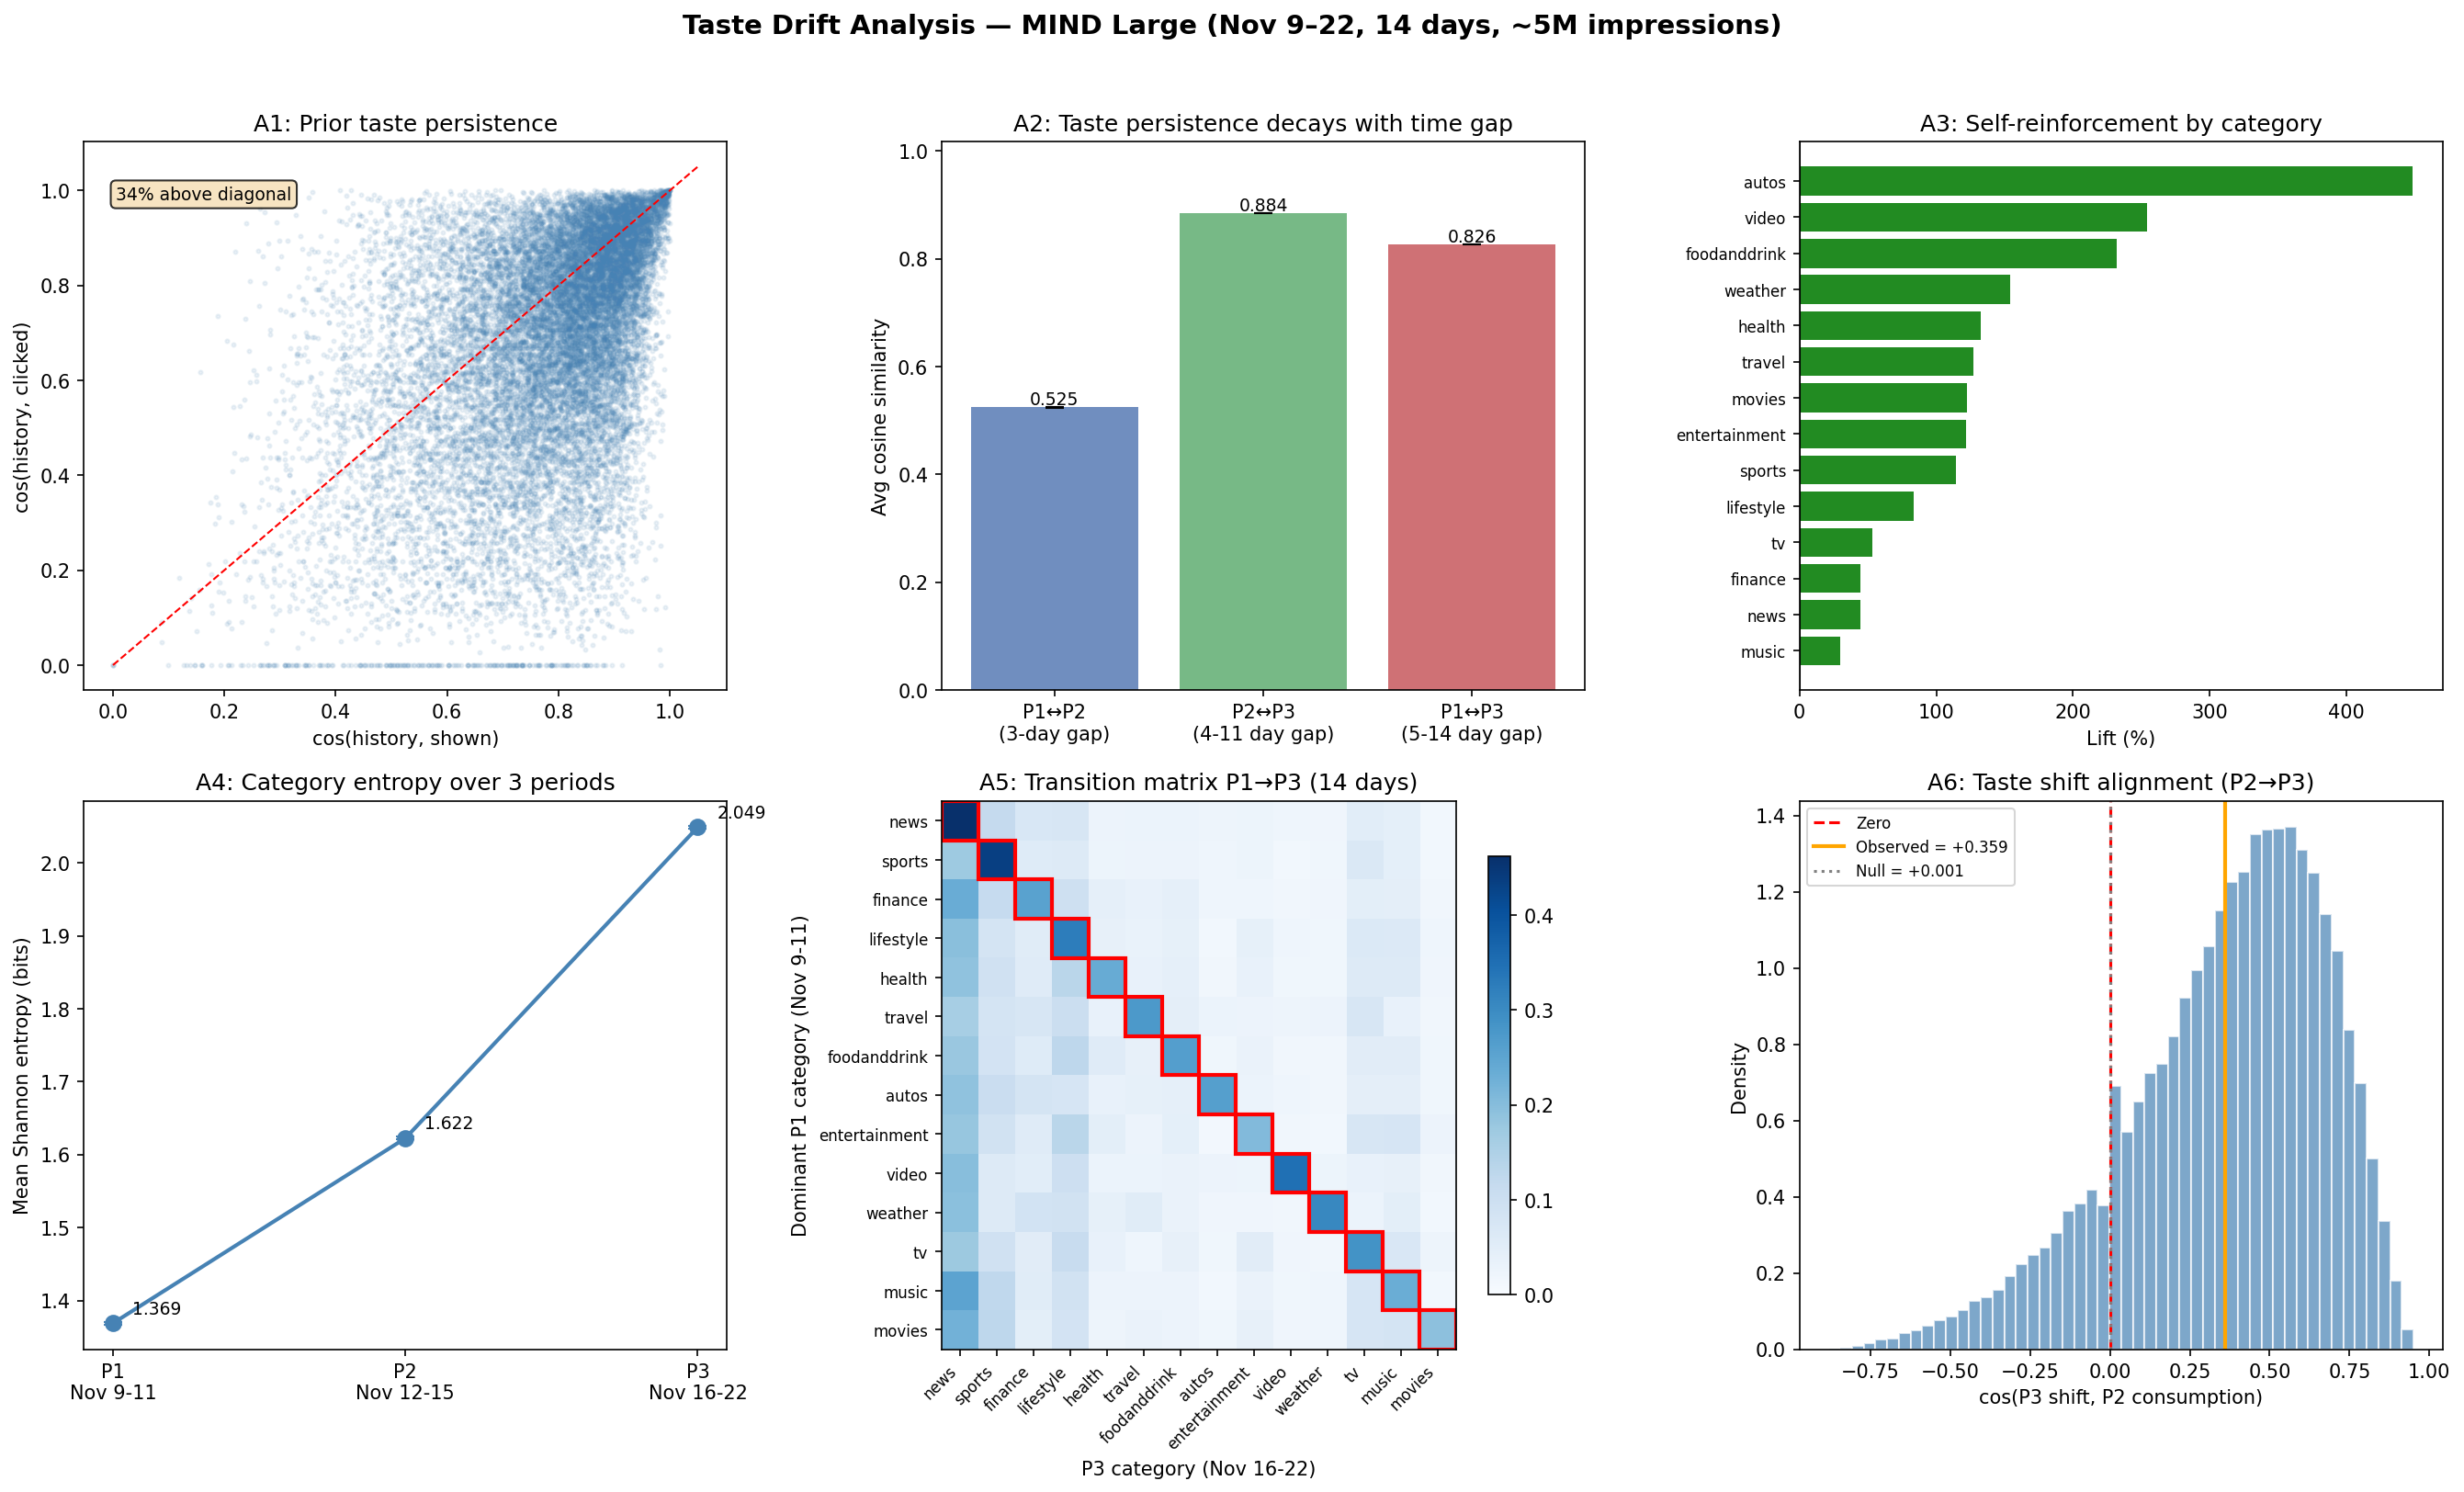
\includegraphics[width=\textwidth]{taste_drift_large.png}
    \caption{Taste drift analysis. (A1)~Prior taste persistence. (A2)~Taste similarity decay across three periods. (A3)~Self-reinforcement lift by category. (A4)~Entropy trajectory P1$\to$P2$\to$P3. (A5)~Transition heatmap P1$\to$P3. (A6)~Taste shift alignment with permutation null.}
    \label{fig:large}
\end{figure}

\begin{figure}[ht]
    \centering
    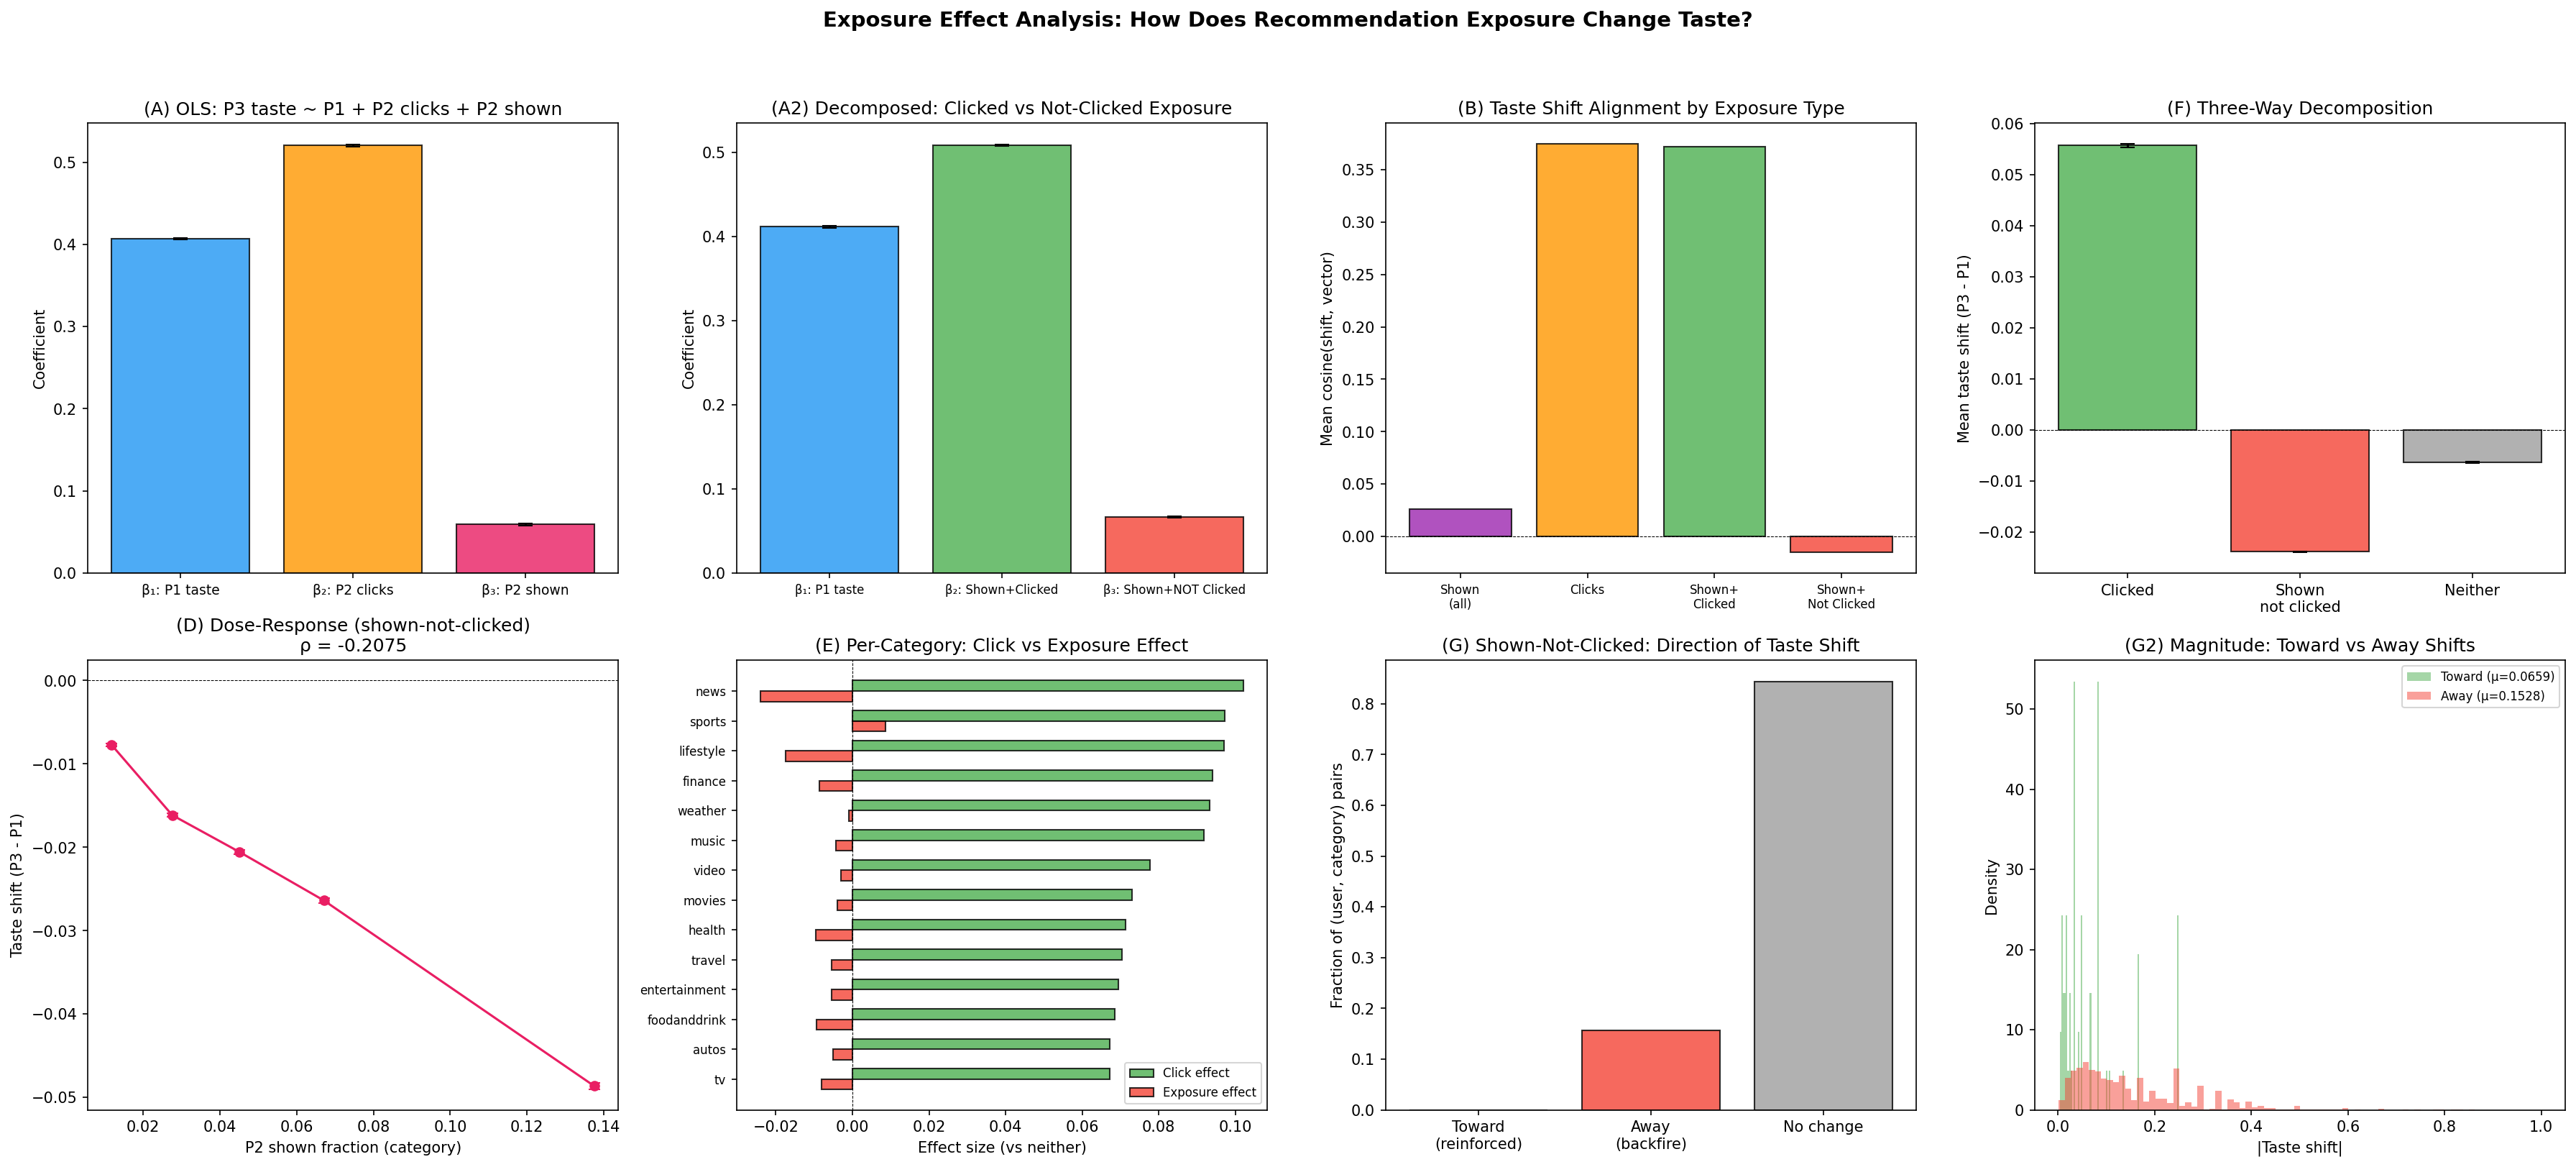
\includegraphics[width=\textwidth]{exposure_effect_full.png}
    \caption{Exposure effect analysis. (A)~OLS coefficients: P3 taste on P1 taste, P2 clicks, P2 shown. (A2)~Decomposed OLS: shown+clicked vs.\ shown+not-clicked. (B)~Cosine alignment of taste shift with four exposure vectors. (F)~Three-way decomposition: clicked gains, shown-not-clicked loses more than baseline. (D)~Dose-response for shown-not-clicked. (E)~Per-category click vs.\ exposure effects. (G)~Direction of shift for shown-not-clicked pairs. (G2)~Magnitude of toward vs.\ away shifts.}
    \label{fig:exposure}
\end{figure}

\end{document}
